\documentclass{article}
\usepackage{graphicx}

\begin{document}
\title{Overview of COMP354 Project}
\author{Team D}
\date{\today}

\maketitle

\section{Vessel Monitoring System}
The Vessel Monitoring System is a Java-based system which listens to incoming radar data from multiple vessels at sea and keeps track of their type, position, and velocity. The goal of the system is to ensure that no vessel ever collide with one another.

To accomplish this, the system will generate appropriate alarms when a dangerous situation arises. Each alarm has a level which corresponds to the degree of danger.

For the sake of testing, the system will also include a \emph{Radar Simulator} which will emulate the behavior of a real vessel. When invoked, the simulator will send fake (but valid) data read from a file to the VMS.

\begin{figure}[h]
\caption{High-level use case of whole system}
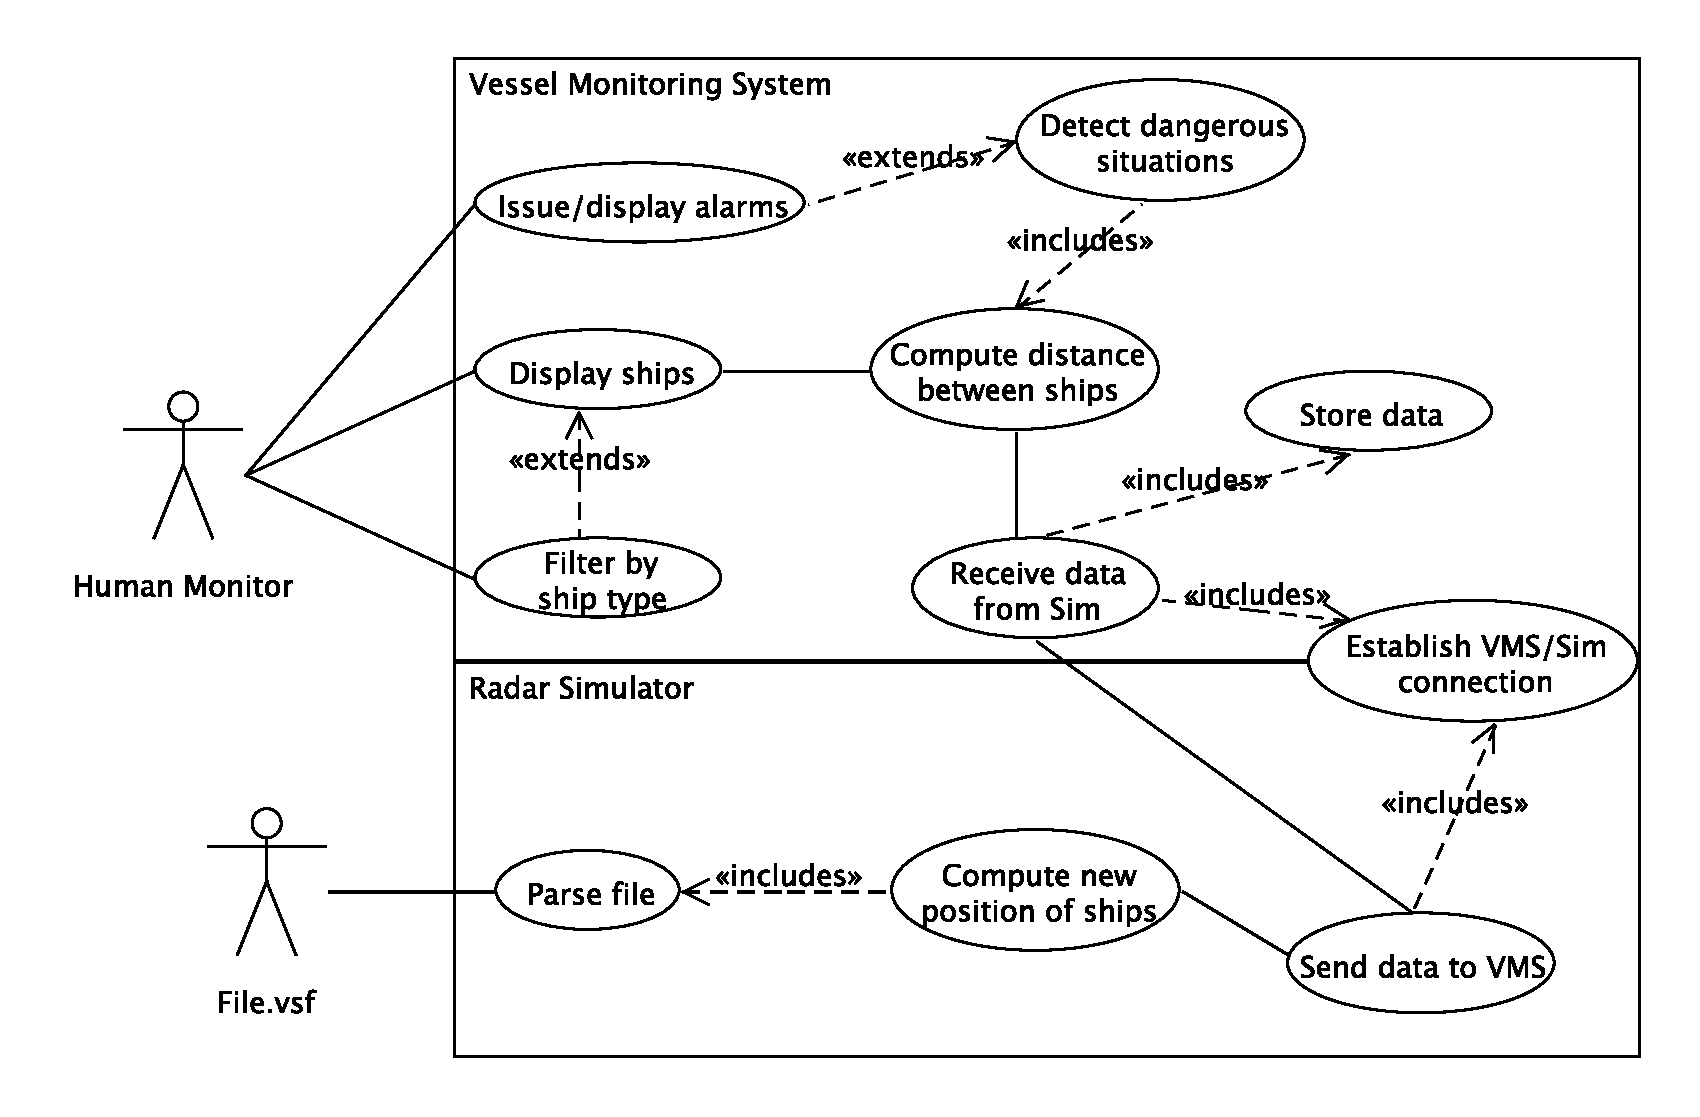
\includegraphics[width=\linewidth]{usecase.eps}
\end{figure}

\section{Team}
Here is the make-up of the team which will implement the system.

\medskip
\begin{center}
\begin{tabular}{| l | c | r |}
\hline
Name & Student ID & Role \\
\hline
\hline
Stefanie Lavoie & 1951750 & Documenter\\
\hline
Pinsonn Laverdure & 9684352 & Documenter\\
\hline
Ghislain Ledoux & 6376320 & Coder\\
\hline
Rigil Malubay & 6262732 & Coder\\
\hline
Philippe Milot & 9164111 & Leader,Documenter \\
\hline
Christopher Mukherjee & 6291929 & Tester\\
\hline
\end{tabular}
\end{center}

\end{document}
